\PassOptionsToPackage{unicode=true}{hyperref} % options for packages loaded elsewhere
\PassOptionsToPackage{hyphens}{url}
\documentclass[11pt,dvipsnames,ignorenonframetext,aspectratio=169]{beamer}
\IfFileExists{pgfpages.sty}{\usepackage{pgfpages}}{}
\setbeamertemplate{caption}[numbered]
\setbeamertemplate{caption label separator}{: }
\setbeamercolor{caption name}{fg=normal text.fg}
\beamertemplatenavigationsymbolsempty
\usepackage{lmodern}
\usepackage{amssymb,amsmath}
\usepackage{ifxetex,ifluatex}
\usepackage{fixltx2e} % provides \textsubscript
\ifnum 0\ifxetex 1\fi\ifluatex 1\fi=0 % if pdftex
  \usepackage[T1]{fontenc}
  \usepackage[utf8]{inputenc}
\else % if luatex or xelatex
  \ifxetex
    \usepackage{mathspec}
  \else
    \usepackage{fontspec}
\fi
\defaultfontfeatures{Ligatures=TeX,Scale=MatchLowercase}







\fi

  \usetheme[]{monash}

  \usecolortheme{monashwhite}


% A default size of 24 is set in beamerthememonash.sty

% Title page
\setbeamertemplate{title page}
{\placefig{-0.01}{-0.01}{width=1.01\paperwidth,height=1.01\paperheight}{1651290829511.jpg}
\begin{textblock}{7.5}(1,2.8)\usebeamerfont{title}
{\color{white}\raggedright\par\inserttitle}
\end{textblock}
\begin{textblock}{7.5}(1,7)
{\color{white}\raggedright{\insertauthor}\mbox{}\\[0.2cm]
\insertdate}
\end{textblock}}


  \useinnertheme{rounded}

  \useoutertheme{smoothtree}

% use upquote if available, for straight quotes in verbatim environments
\IfFileExists{upquote.sty}{\usepackage{upquote}}{}
% use microtype if available
\IfFileExists{microtype.sty}{%
  \usepackage{microtype}
  \UseMicrotypeSet[protrusion]{basicmath} % disable protrusion for tt fonts
}{}


\newif\ifbibliography
  \usepackage[round]{natbib}
  \bibliographystyle{plainnat}


\hypersetup{
      pdftitle={Spatial data management and geodesy},
            colorlinks=true,
    linkcolor=red,
    citecolor=Blue,
    urlcolor=pink,
    breaklinks=true}
%\urlstyle{same}  % Use monospace font for urls







% Prevent slide breaks in the middle of a paragraph:
\widowpenalties 1 10000
\raggedbottom

  \AtBeginPart{
    \let\insertpartnumber\relax
    \let\partname\relax
    \frame{\partpage}
  }
  \AtBeginSection{
    \ifbibliography
    \else
      \let\insertsectionnumber\relax
      \let\sectionname\relax
      \frame{\sectionpage}
    \fi
  }
  \AtBeginSubsection{
    \let\insertsubsectionnumber\relax
    \let\subsectionname\relax
    \frame{\subsectionpage}
  }



\setlength{\parindent}{0pt}
\setlength{\parskip}{6pt plus 2pt minus 1pt}
\setlength{\emergencystretch}{3em}  % prevent overfull lines
\providecommand{\tightlist}{%
  \setlength{\itemsep}{0pt}\setlength{\parskip}{0pt}}

  \setcounter{secnumdepth}{0}


%% Monash overrides
\AtBeginSection[]{
   \frame<beamer>{
   \frametitle{Outline}\vspace*{0.2cm}
   
   \tableofcontents[currentsection,hideallsubsections]
  }}

% Redefine shaded environment if it exists (to ensure text is black)
\ifcsname Shaded\endcsname
  \definecolor{shadecolor}{RGB}{225,225,225}
  \renewenvironment{Shaded}{\color{black}\begin{snugshade}\color{black}}{\end{snugshade}}
\fi
%%


  \usepackage{setspace}
  \usepackage{wasysym}
  % \usepackage{footnote} % don't use this this breaks all
  \usepackage{fontenc}
  \usepackage{fontawesome}
  \usepackage{booktabs,siunitx}
  \usepackage{longtable}
  \usepackage{array}
  \usepackage{multirow}
  \usepackage{wrapfig}
  \usepackage{float}
  \usepackage{colortbl}
  \usepackage{pdflscape}
  \usepackage{tabu}
  \usepackage{threeparttable}
  \usepackage{threeparttablex}
  \usepackage[normalem]{ulem}
  \usepackage{makecell}
  \usepackage{xcolor}
  \usepackage{tikz} % required for image opacity change
  \usepackage[absolute,overlay]{textpos} % for text formatting
  \usepackage{chemfig}
  \usepackage[skip=0.333\baselineskip]{caption}
  % \newcommand*{\AlignChar}[1]{\makebox[1ex][c]{\ensuremath{\scriptstyle#1}}}%

  % this font option is amenable for beamer
  \setbeamerfont{caption}{size=\tiny}
  \singlespacing
  \definecolor{lightgrayd}{gray}{0.95}
  \definecolor{skyblued}{rgb}{0.65, 0.6, 0.94}
  \definecolor{oranged}{RGB}{245, 145, 200}

  % \newlength{\cslhangindent}
  % \setlength{\cslhangindent}{1.5em}
  % \newenvironment{cslreferences}%
  %   {\setlength{\parindent}{0pt}%
  %   \everypar{\setlength{\hangindent}{\cslhangindent}}\ignorespaces}%
  %   {\par}


  \newcommand{\bcolumns}{\begin{columns}[T, onlytextwidth]}
  \newcommand{\ecolumns}{\end{columns}}

  \newcommand{\bdescription}{\begin{description}}
  \newcommand{\edescription}{\end{description}}

  \newcommand{\bitemize}{\begin{itemize}}
  \newcommand{\eitemize}{\end{itemize}}
  \AtBeginSubsection{}

  \title[]{Spatial data management and geodesy}


  \author[
        Deependra Dhakal\\
Assistant Professor\\
\textit{ddhakal.rookie@gmail.com}\\
\url{https://rookie.rbind.io}
    ]{Deependra Dhakal\\
Assistant Professor\\
\textit{ddhakal.rookie@gmail.com}\\
\url{https://rookie.rbind.io}}


\date[
      
  ]{
    }

\begin{document}

% Hide progress bar and footline on titlepage
  \begin{frame}[plain]
  \titlepage
  \end{frame}


   \frame<beamer>{
   \frametitle{Outline}\vspace*{0.2cm}
   
   \tableofcontents[hideallsubsections]
  }

\hypertarget{geodesy}{%
\section{Geodesy}\label{geodesy}}

\begin{frame}{}
\protect\hypertarget{section}{}
\bcolumns
\column{0.62\textwidth}

\begin{figure}
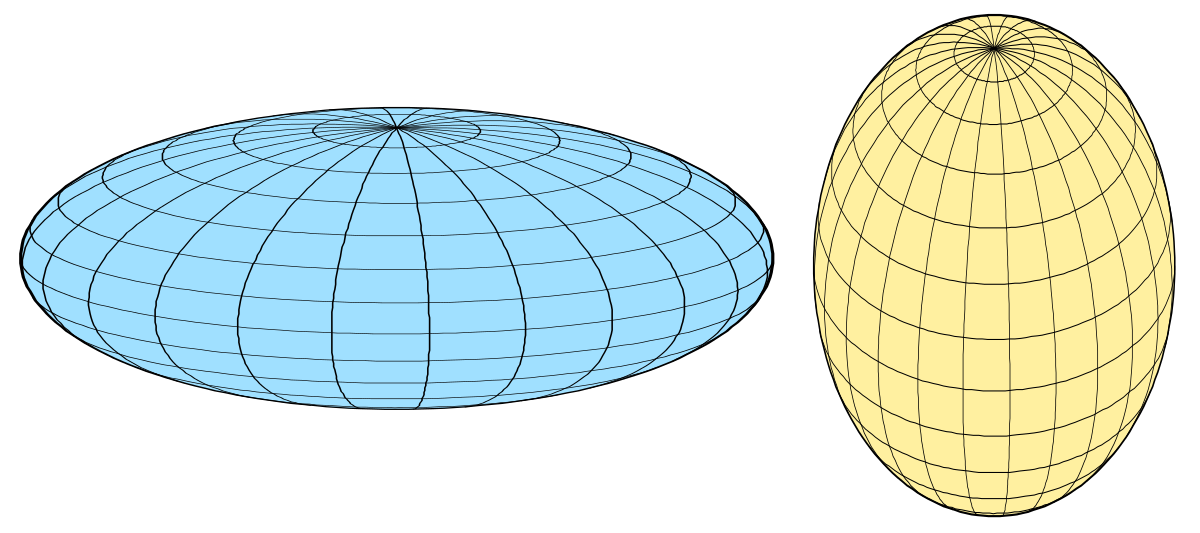
\includegraphics[width=0.84\linewidth]{../images/spheroids_prolate_oblate} \caption{Geometric models for early earth. Cassinis family postulated that earth was prolate (right). Sir Issac Newton hypothesized that earth, with its rotation around equatorial axis was oblate (left). Newton's concept was later verified in the course of French Geodesic Mission to Equator and to the Lapland (Source: \url{https://en.wikipedia.org/wiki/French_Geodesic_Mission_to_the_Equator}, \url{https://en.wikipedia.org/wiki/French_Geodesic_Mission_to_Lapland}).}\label{fig:earth-geometric-models}
\end{figure}

\column{0.35\textwidth}

\begin{figure}
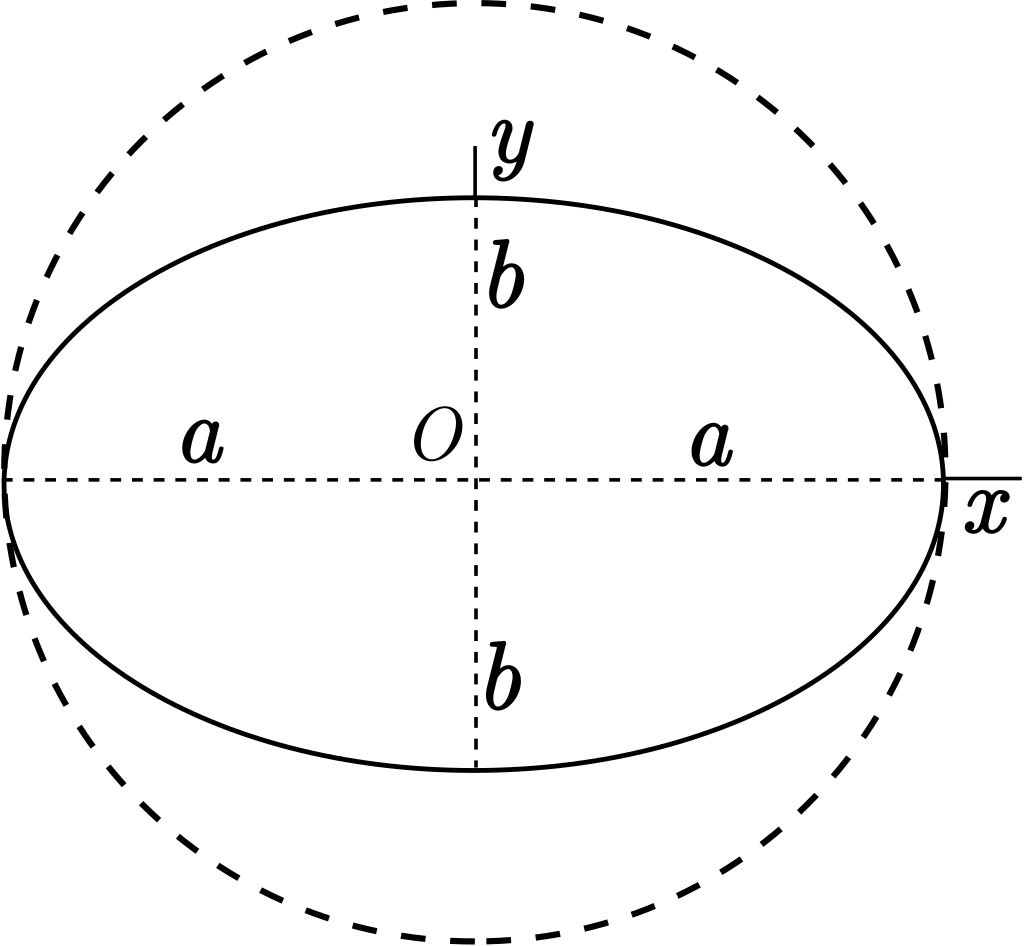
\includegraphics[width=0.7\linewidth]{../images/an_ellipse_with_auxiliary_circle.svg} \caption{An ellipse constructed by compressing a circle of radius a labelled with terms indicating major (a) and minor (b) axis.}\label{fig:ellipse-with-auxiliary-circle}
\end{figure}

\ecolumns

\footnotesize

\begin{itemize}
\tightlist
\item
  Flattening (first type; Geodetic reference ellipsoids are specified by
  giving \(\frac{1}{f}\)) is defined as,
\end{itemize}

\[
\small
f = \frac{(a-b)}{a}
\]
\end{frame}

\begin{frame}{Geodetic datum}
\protect\hypertarget{geodetic-datum}{}
\bcolumns
\column{0.7\textwidth}
\footnotesize

\begin{itemize}
\tightlist
\item
  A set of constants specifying the coordinate system used for geodetic
  control, i.e., for calculating coordinates and elevations of points on
  the Earth.
\item
  Specific geodetic datums are usually given distinctive names. (e.g.,
  North American Datum of 1983, Old Hawaiian Datum, National Geodetic
  Vertical Datum of 1929, etc.)
\item
  Characterized by some realization:

  \begin{itemize}
  \scriptsize
  \item a set of passive and/or active physical monuments with published horizontal and/or vertical coordinates
  \end{itemize}
\end{itemize}

\column{0.3\textwidth}

\begin{figure}
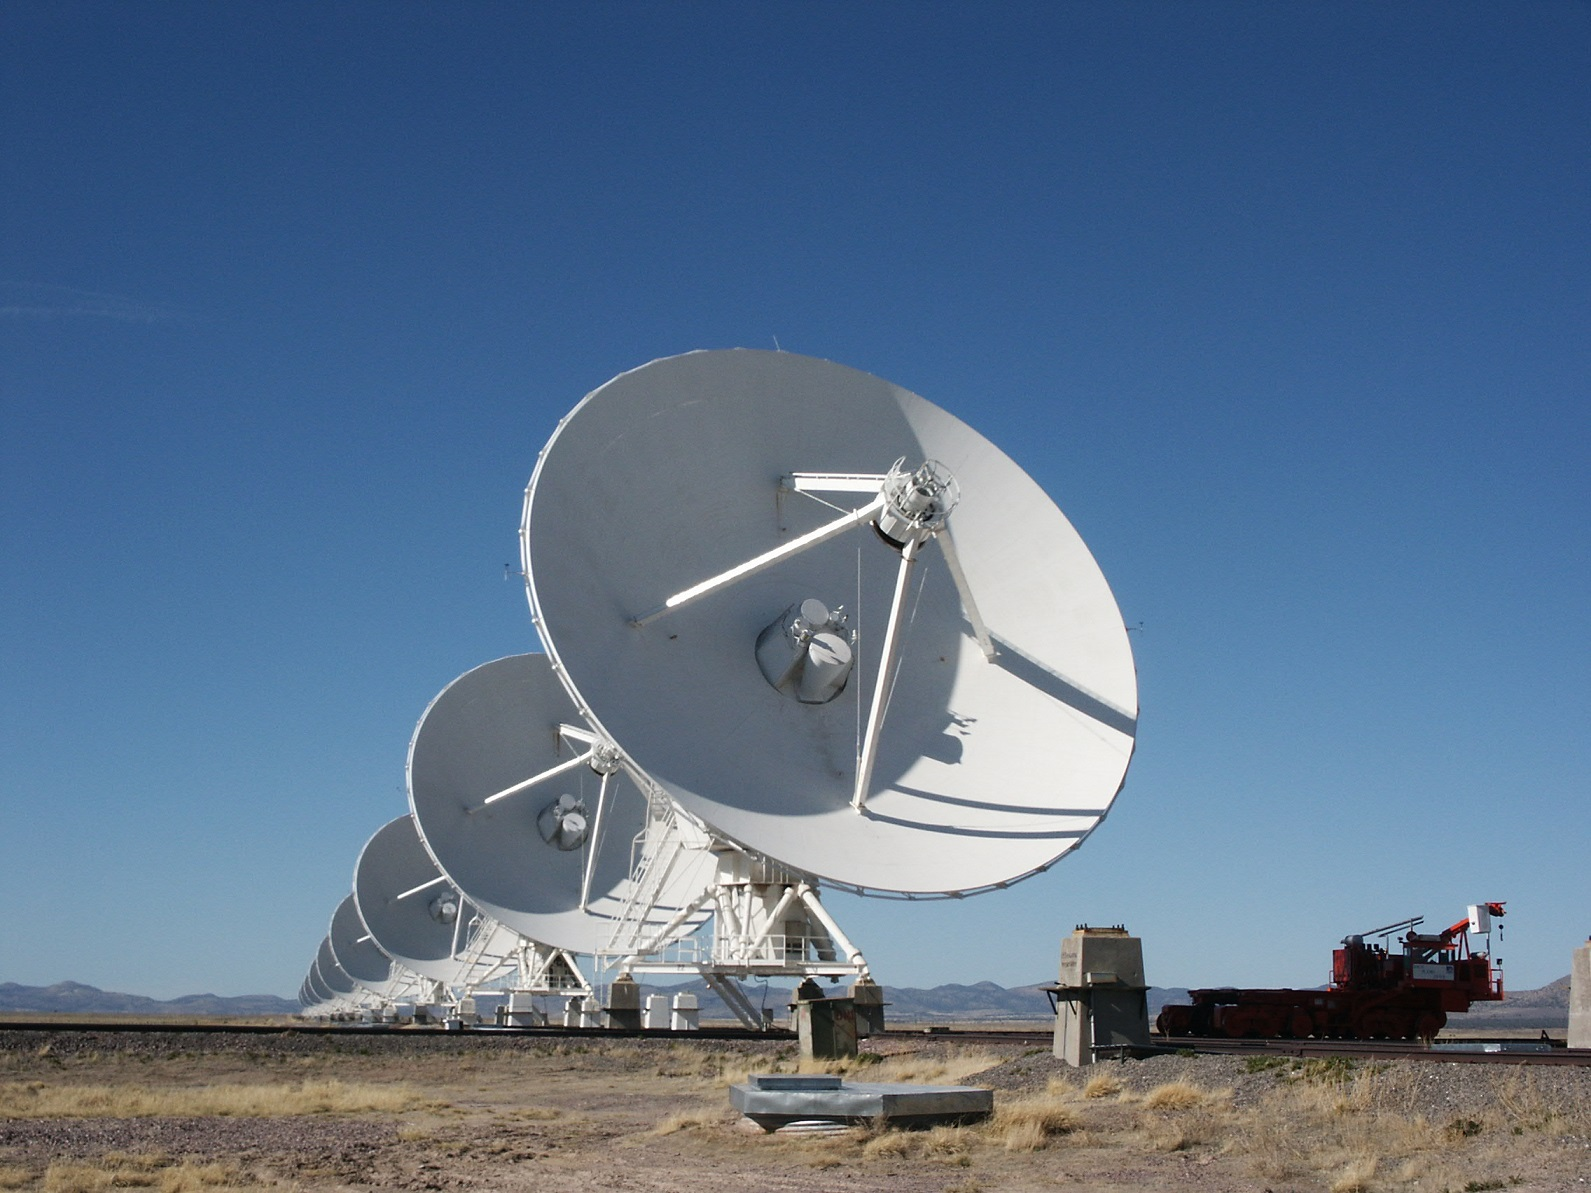
\includegraphics[width=0.98\linewidth]{../images/vlbi_satellite} \caption{VLBI satellite.}\label{fig:vlbi-satellite}
\end{figure}

\ecolumns
\end{frame}

\begin{frame}{}
\protect\hypertarget{section-1}{}
\begin{itemize}
\tightlist
\item
  Reference system is the idealized concepts of an ideal ellipsoid,
  coordinate system origin, and Earth orientation (Chandler wooble),
  nutation, precession and plate tectonics.
\item
  Reference frame is the realization of the reference system through
  observation.

  \begin{itemize}
  \scriptsize
  \item GNSS (Global Navigation Satellite System)
  \item VLBI (Very Long Baseline Interferometry)
  \item SLR
  \end{itemize}
\item
  Definition and implementation of the reference systems and frame is
  currently entrusted upon the International Earth Rotation and
  Reference System Service (IERS)
\end{itemize}
\end{frame}

\begin{frame}{Horizontal and vertical datum}
\protect\hypertarget{horizontal-and-vertical-datum}{}
\begin{itemize}
\tightlist
\item
  Horizontal/geometric datums

  \begin{itemize}
  \tightlist
  \item
    8 basic constants

    \begin{itemize}
    \tightlist
    \item
      3 specify the location of the origin of the coordinate system
    \item
      3 specify the orientation of the coordinate system
    \item
      2 specify the dimensions of the reference ellipsoid
    \end{itemize}
  \end{itemize}
\item
  Vertical datums

  \begin{itemize}
  \tightlist
  \item
    Set of fundamental elevations to which other elevations are referred
  \end{itemize}
\end{itemize}
\end{frame}

\begin{frame}{Tidal and geodetic datum}
\protect\hypertarget{tidal-and-geodetic-datum}{}
\begin{description}
\item[Tidal] Defined by observation of tidal variations over some period of time (MSL, MLLW, MLW, MHW, MHHW, etc.)
\item[Geodetic] Either directly or loosely based on Mean Sea Level at one or more points at some epoch (NGVD 29, NAVD 88, IGLD85, etc.)
\end{description}
\end{frame}

\begin{frame}{The Geoid}
\protect\hypertarget{the-geoid}{}
\begin{itemize}
\tightlist
\item
  An equipotential surface to which gravity is normal and most closely
  approximates Mean Sea Level over the entire Earth.
\end{itemize}

\begin{figure}
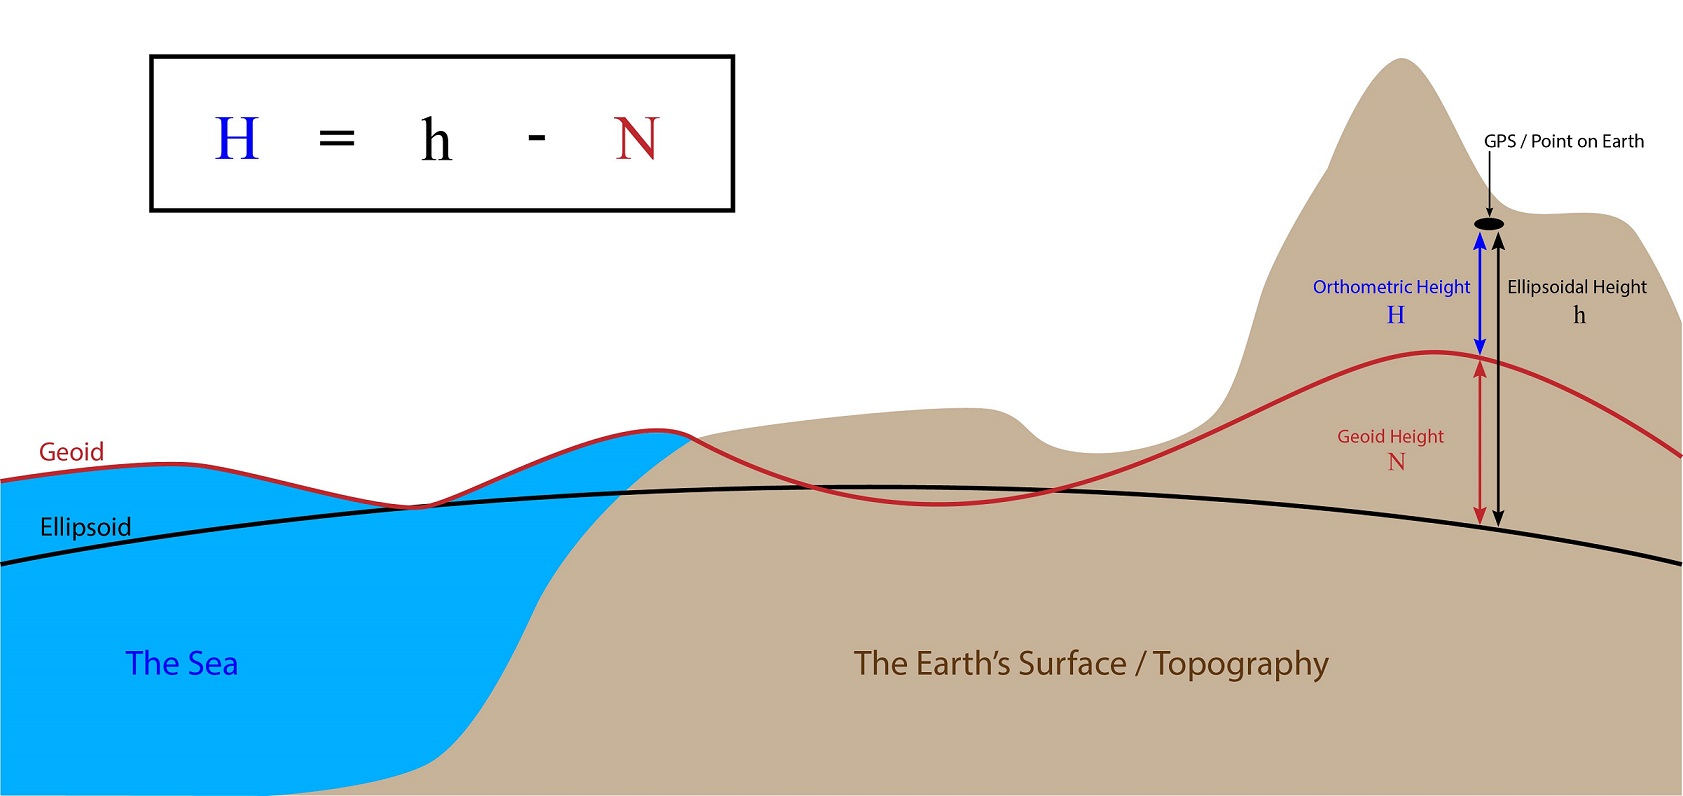
\includegraphics[width=0.7\linewidth]{../images/geoid-ellipsoid-relationship} \caption{Relationship between the Ellipsoid and the Geoid. H = Orthometric height (NAD 88), h = Ellipsoid height (NAD 83 (2011)), N = Geoid height (GEOID12A/B)}\label{fig:geoid-ellipsoid-relationship}
\end{figure}
\end{frame}

\hypertarget{geospatial-data}{%
\section{Geospatial data}\label{geospatial-data}}

\begin{frame}{Spatial data}
\protect\hypertarget{spatial-data}{}
\begin{itemize}
\tightlist
\item
  \alert{Spatial data} describes the absolute and relative location of
  geographic features.
\item
  Spatial data consists of points, lines, polygons or other geographic
  and geometric data primites that we can map by location.
\item
  Two forms of spatial data each providing information connected to
  geographical locations are:

  \begin{itemize}
  \tightlist
  \item
    Vector data
  \item
    Raster data
  \end{itemize}
\item
  Data describing the characteristics of geographical features included
  in the spatial data is called \alert{attribute data}.

  \begin{itemize}
  \tightlist
  \item
    in combination with spatial information, attribute of geographical
    features provide meaningful insights from a map.
  \item
    attributes could relate to: characteristics of soil, soil type,
    elevation, rock type, vegetation type, thematic summary relating to
    certain aspects of the crop/vegetation.
  \end{itemize}
\end{itemize}
\end{frame}

\begin{frame}{}
\protect\hypertarget{section-2}{}
\begin{figure}
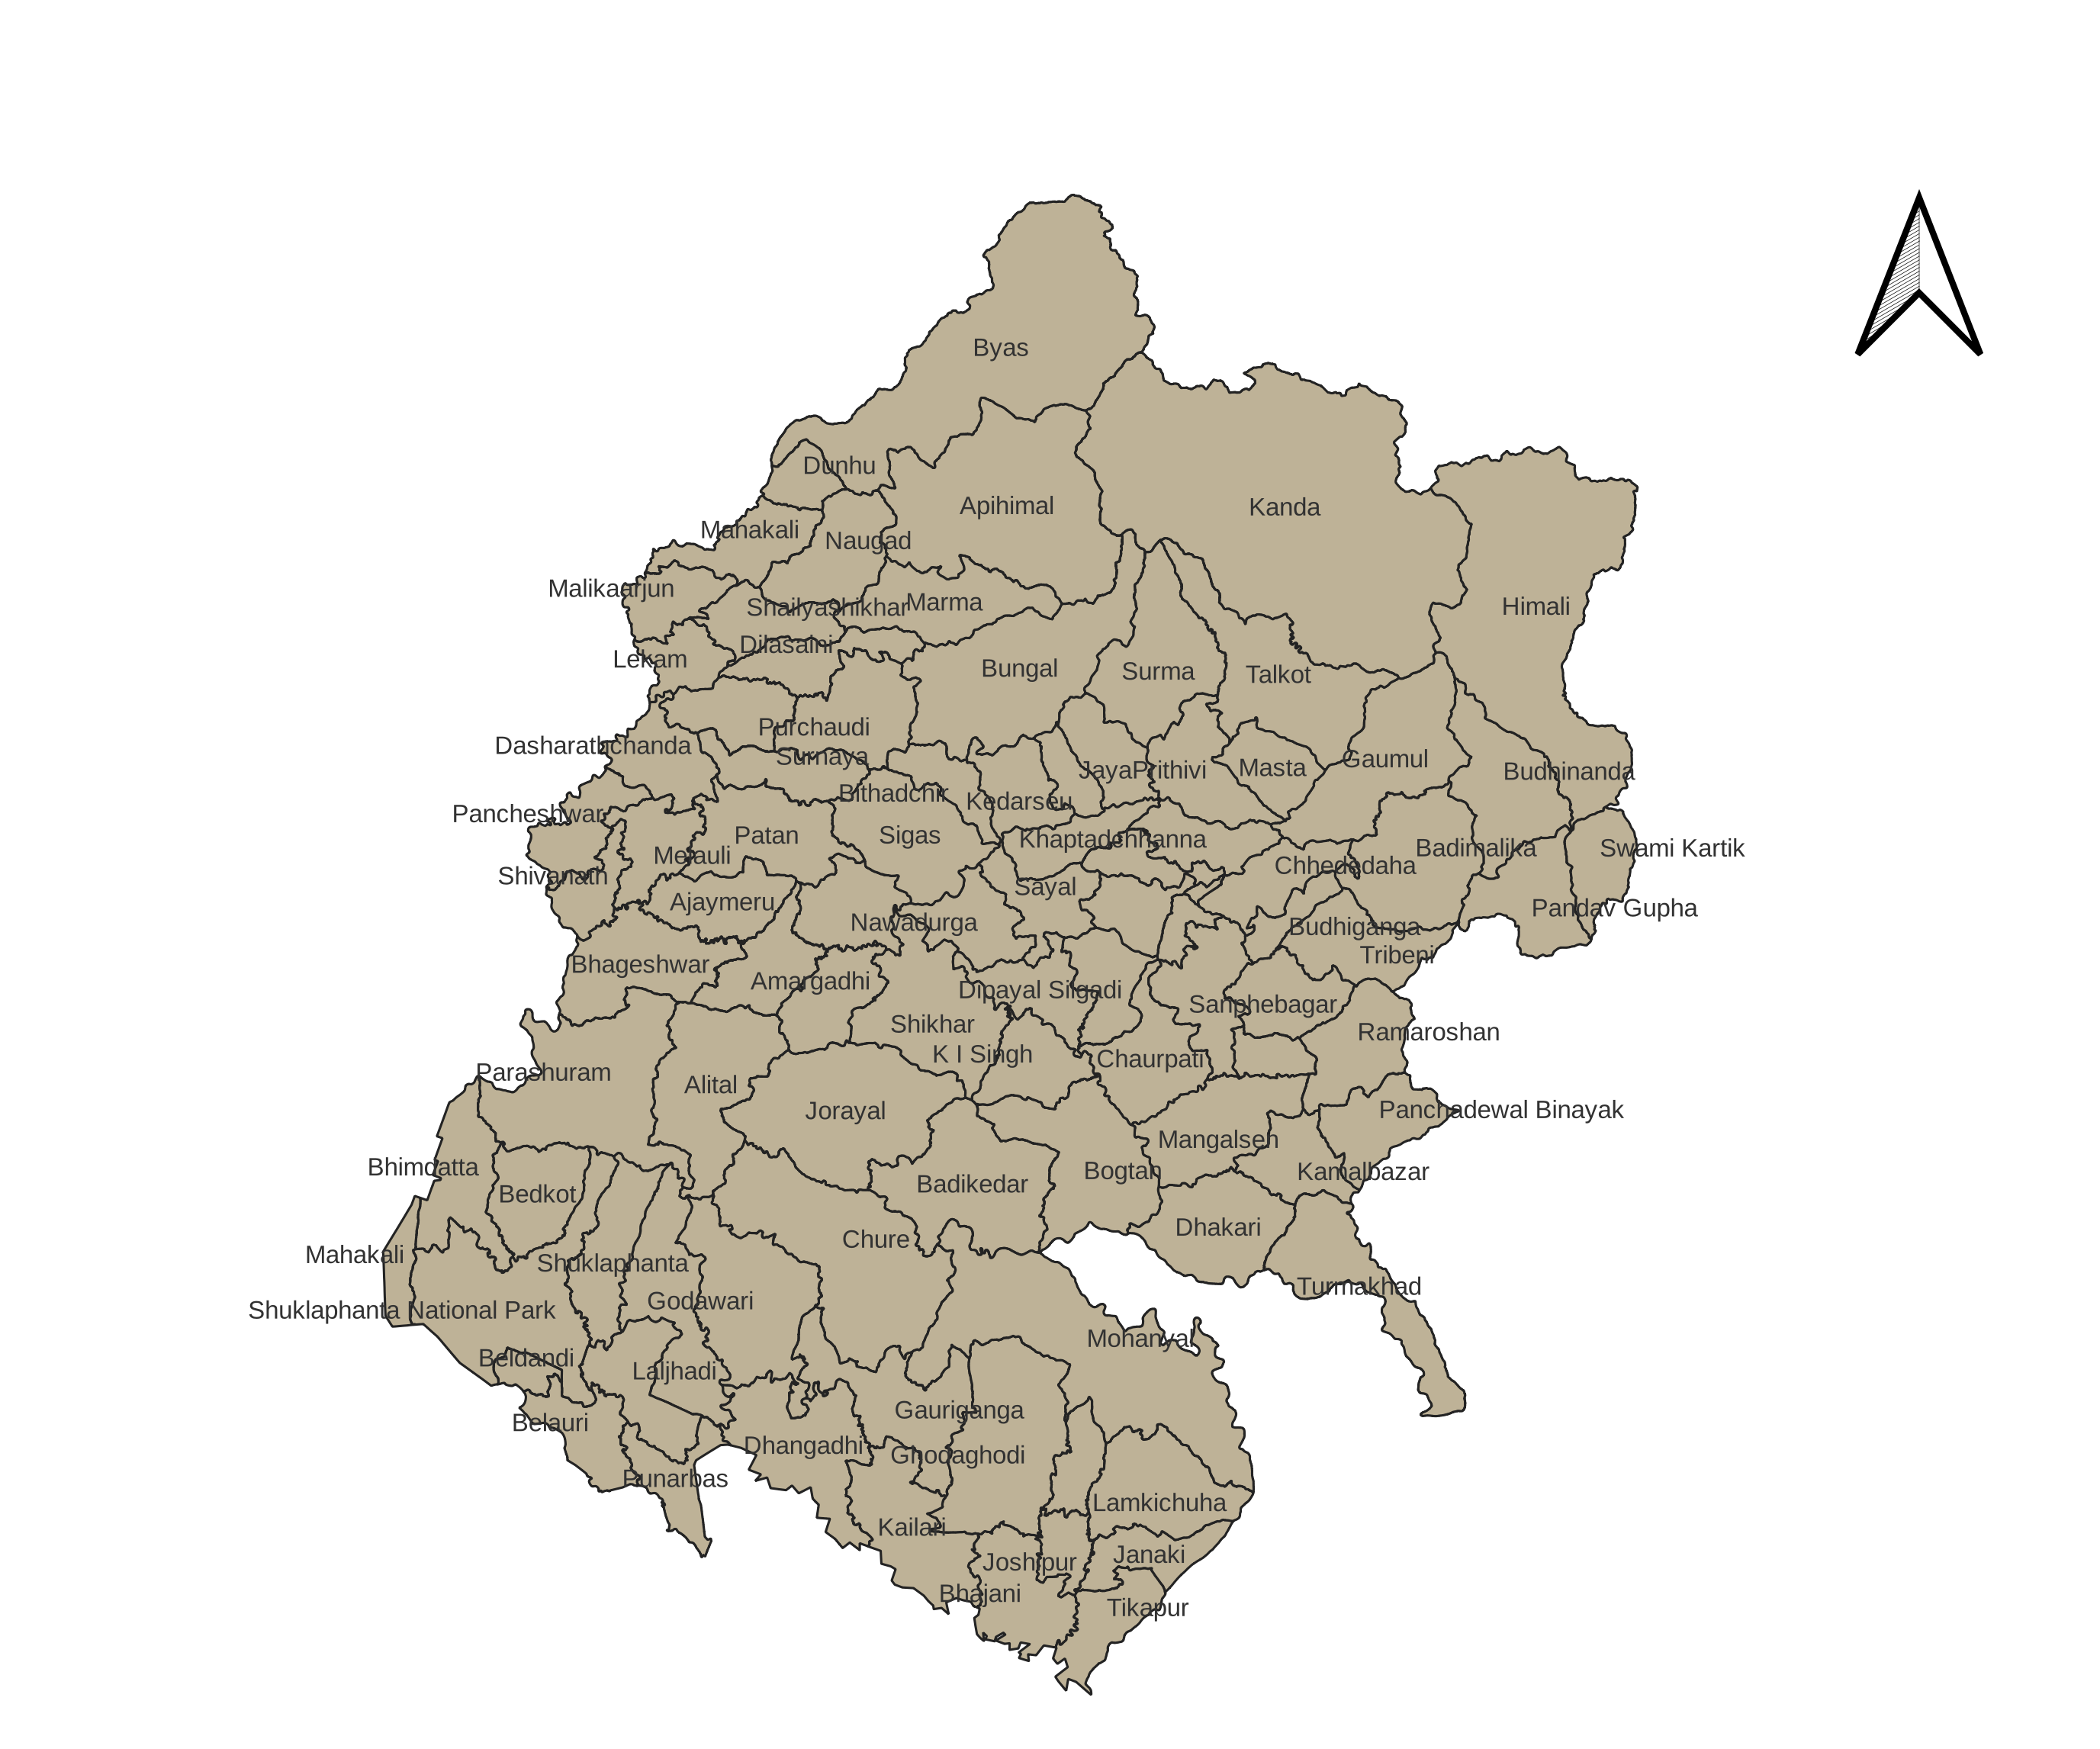
\includegraphics[width=0.55\linewidth]{../images/sudurpaschim_LU_labelled} \caption{An exported form of vector data stored as Shapefile showing areas of Sudurpaschim province of Nepal.}\label{fig:spatial-raster-data}
\end{figure}

\footnotesize

\begin{itemize}
\tightlist
\item
  Refer to `../data/artificial\_points\_polygon' directory for
  demonstration.
\end{itemize}
\end{frame}

\begin{frame}{}
\protect\hypertarget{section-3}{}
\begin{itemize}
\tightlist
\item
  In vector data model, feature boundaries are converted to
  straight-sided polygons that approximate the original regions. These
  polygons are encoded by determining the coordinates of their vertices,
  called points or nodes, which can be connected to form lines or arcs.
\item
  Topological coding includes ``intelligence'' in the data structure
  relative to the spatial relationship (connectivity and adjacency)
  among features

  \begin{itemize}
  \tightlist
  \item
    it keeps track of which arcs share common nodes and what polygons
    are to the left and right of a given arc
  \end{itemize}
\item
  Vector data encoding allows for spatial operations such as overlay
  analysis, buffering, and network analysis.
\item
  Allows for lower data volume, better spatial resolution, and the
  preservation of topological data relationships (allowing efficient
  network analysis)
\end{itemize}
\end{frame}

\begin{frame}{Raster data}
\protect\hypertarget{raster-data}{}
\begin{itemize}
\tightlist
\item
  Raster systems generally have simpler data structures

  \begin{itemize}
  \tightlist
  \item
    afford greater computational efficiency in such operations as
    overlay analysis
  \item
    represent features having high spatial variability and/or `blurred
    boundaries' (e.g., between pure and mixed vegetation zones)
    effectively
  \end{itemize}
\item
  Limitations

  \begin{itemize}
  \tightlist
  \item
    volumes are relatively greater
  \item
    spatial resolution of the data is limited to the size of the cells
    comprising the raster
  \item
    topological relationships among features are more difficult to
    represent
  \end{itemize}
\item
  Digital remote sensing images are collected in a raster format,
  accordingly they are inherently compatible with other sources of
  information in a raster domain
\item
  Image processing procedures as automated land cover classification
  result in the creation of interpreted or derived data files in a
  raster format. These derived data are again inherently compatible with
  the other sources of data represented in a raster format.
\end{itemize}
\end{frame}

\begin{frame}{}
\protect\hypertarget{section-4}{}
\bcolumns
\column{0.6\textwidth}

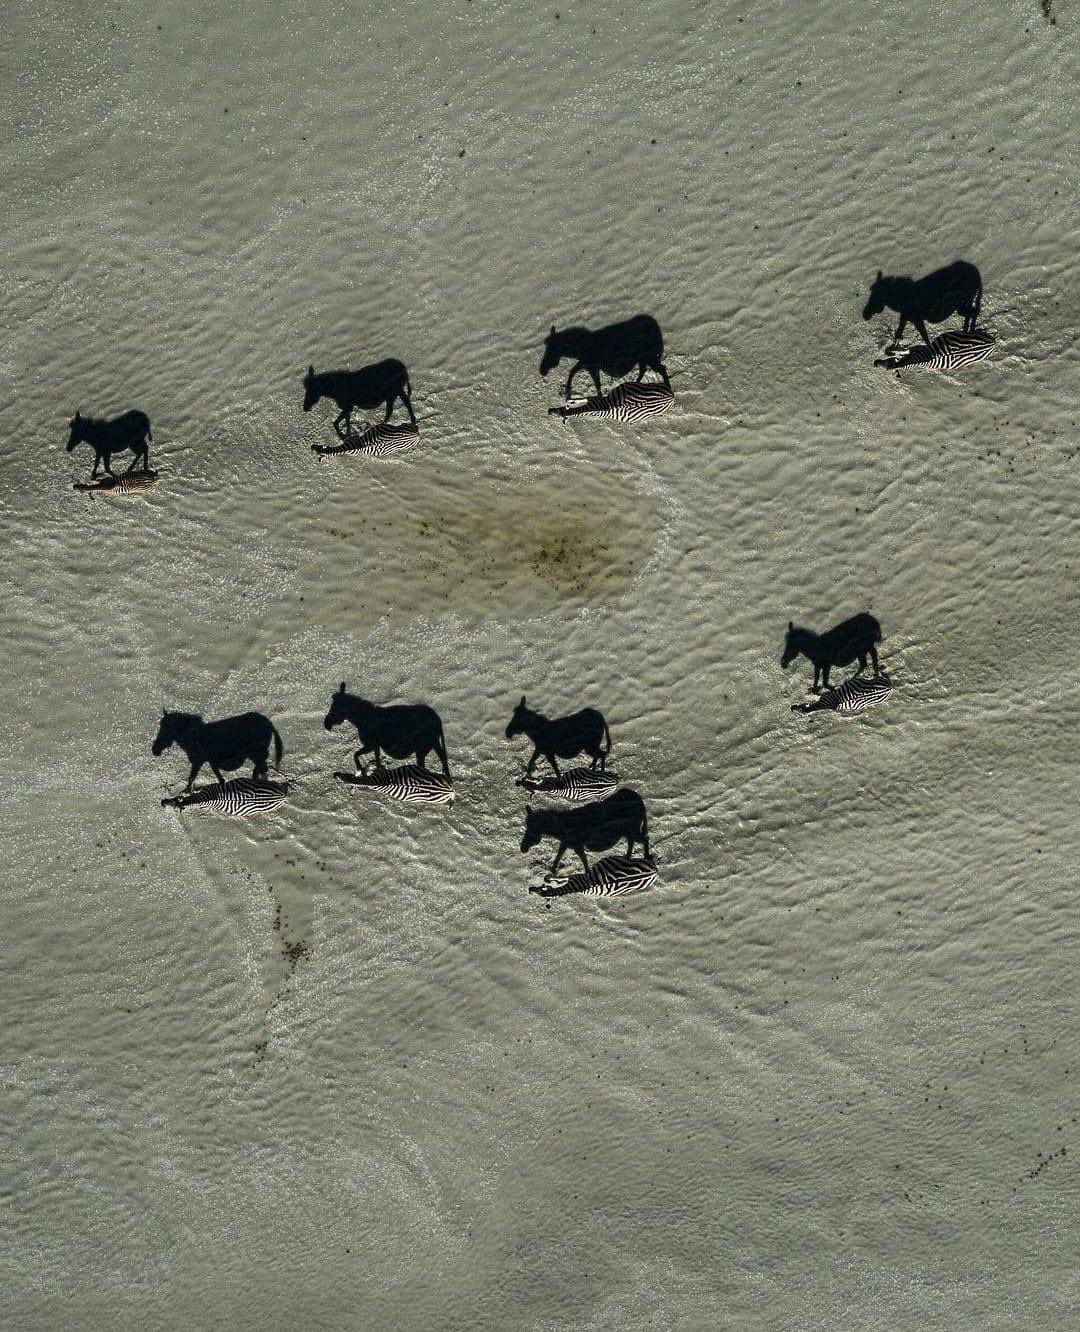
\includegraphics[width=0.64\linewidth]{../images/zebra_herd_super_big}

\column{0.4\textwidth}

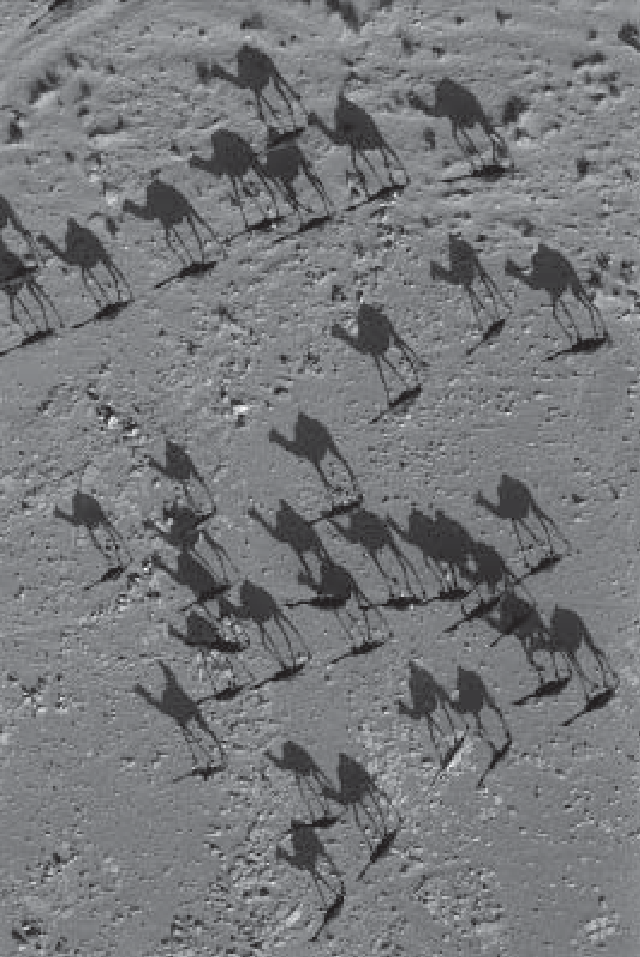
\includegraphics[width=0.62\linewidth]{../images/camel_vertical}

\ecolumns
\end{frame}

\begin{frame}{Free gis data}
\protect\hypertarget{free-gis-data}{}
\url{https://freegisdata.rtwilson.com/}
\end{frame}

\begin{frame}{Spatial dataset: An example}
\protect\hypertarget{spatial-dataset-an-example}{}
\includegraphics[width=0.6\linewidth]{06.7-spatial_data_management_geodesy_files/figure-beamer/example-data-1}
\end{frame}

\begin{frame}{}
\protect\hypertarget{section-5}{}
\url{https://erinbecker.github.io/r-raster-vector-geospatial/aio.html}
\end{frame}

\hypertarget{bibliography}{%
\section{Bibliography}\label{bibliography}}

\begin{frame}{References}
\protect\hypertarget{references}{}
\end{frame}

          \begin{frame}[allowframebreaks]{}
    \bibliographytrue
    \bibliography{./../bibliographies.bib}
    \end{frame}
  


\end{document}
